% ---- ETD Document Class and Useful Packages ---- %
\documentclass{ucetd}
\usepackage{subfigure,epsfig,amsfonts}
\usepackage{natbib}
\usepackage{amsmath}
\usepackage{amssymb}
\usepackage{amsthm}
\usepackage[toc,page]{appendix}
\usepackage[labelfont=bf]{caption}
\usepackage{rotating}
\usepackage[dvipsnames]{xcolor}

\usepackage{url}
 

%% Use these commands to set biographic information for the title page:
\title{Towards a theory of spatiotemporal correlation transfer in plastic neuronal networks}
\author{Clayton W. Seitz}
\department{Graduate Program in Biophysics}
\division{Physical and Biological Sciences}
\degree{Master of Science}
\date{Winter 2021}

%% Use these commands to set a dedication and epigraph text

\epigraph{Epigraph}

\begin{document}
%% Basic setup commands
% If you don't want a title page comment out the next line and uncomment the line after it:
\maketitle
%\omittitle

% These lines can be commented out to disable the copyright/dedication/epigraph pages
\makecopyright
%\makededication
\makeepigraph


%% Make the various tables of contents
\tableofcontents
%\listoffigures
%\listoftables

%\acknowledgments
% Enter Acknowledgements here

\abstract

A central goal in computational neuroscience is to explain how functional brain states emerge from the complex interactions of excitatory and inhibitory neurons. Recent years have hosted many efforts to decode the complex patterns of action potentials in response to sensory stimuli by examining the cross-covariance of neural spike trains. The dynamics of the membrane potential of a neuron embedded in a complex network is determined by many factors including network topology, homeostasis, and noise. At the same time, the network topology is not static. Synaptic plasticity allows neural circuits to guide their own topological evolution and certain plasticity mechanisms can drive the formation of functional circuits in response to stimuli. Recently, mathematical methods for quantifying the relationship of network topology and spike train cross-covariance based on mean-field theory and linear response theory have been developed. The application of these tools to plastic networks of neurons holds great promise for improving our understanding of functional brain states and the principles of neural computation. However, their application to the structural changes induced in spatially extended networks, as opposed to those which are connected logically, is largely unexplored. A theoretical understanding of the effect of heterosynaptic and homosynaptic plasticity in response to spatially and temporally correlated stimuli could be of great value. In this thesis, I propose a possible extension of existing models which accounts for the spatial organization of neural circuits and the topological effects of biologically-realistic plasticity rules. This extension would serve to improve our understanding of the functional interaction between membrane potential dynamics and the dynamics of network structure in brain-like network topologies.
\clearpage

\mainmatter

\chapter{Towards a theory of spatiotemporal correlation transfer in plastic neuronal networks}

The thesis has been divided into two primary sections. The first section paints a broad picture of the theoretical techniques that can be used to analyze spike train cross correlations as well as their mathematical connections to network structure. In addition, this section summarizes the mathematical machinery that can relate network dynamics to synaptic plasticity. The primary goal of the first section as a whole is to lay out a necessary set of tools for the project outline laid out at the start of the second section. In addition, the second section contains the results from a set of rudimentary simulations. The scope of these simulations is necessarily narrow. Significant computational advances are needed in order for the simulations to fully connect with the theory presented in the first section. Nevertheless, they do form a basic substrate for future work.

\section{Introduction}

Complex systems are ubiquitous in nature yet our scientific efforts have thus far only begun to gain traction on their governing principles. Complex systems often exihibit behaviors that simply cannot be explained by any of the components in isolation but rather arise from their interactions, bringing emergent phenomena into the focus of modern science. The human brain exemplifies this complexity, thought to consist of billions of noisy neurons, yet the dynamics of these neurons simulataneously maintain an order evident in the stability of our sensory percepts. Furthermore, a central goal of modern neuroscience is to explain how functional brain states emerge from the interactions of dozens, perhaps hundreds, of brain regions, each containing its own complex subnetworks.  These subnetworks can themselves contain thousands of cells, each neuron having on the order of thousands of synaptic connections to other cells within the local network (Binzegger 2004).

It is well accepted that information processing in the brain like sensory, motor, and cognitive functions are carried out by the communication between individual neurons, formally referred to as a \emph{population code}. Amongst a wide variety of cell types, the dominating information processing unit in neocortex is the spiking neuron - a  cell which exhibits transient depolarization and repolarization of the plasma membrane called action potentials or \emph{spikes}.  Neurons in cortex connect when afferent nerve fibers of one cell meet the dendritic tree or soma of another, forming the synapse. The complexity of the structure of neural networks therefore arises from the complex wiring of these communication channels. It is a great challenge to understand how local circuits in the brain interact with sensory stimuli to carry out their dedicated functions.

Early models of neural networks were often deterministic; however, an increasing body of experimental data suggests that neurons, synapses, and systems of neurons are inherently stochastic (Buesing, 2011). The enormous number of degrees of freedom of just a single cell due to millions of unreliable ion channels and synaptic machinery demands a stochastic model for network dynamics (Cannon, 2010; Tuckwell, 1989). Indeed, it has been argued that the variability in neural responses to stimuli and the irregularity of spike-timing owe their origins to noise in the synaptic integration process (Azouz, 1999). Accordingly, some of the most mature models of network dynamics describe the averages of dynamical quantities and/or involve the solution of stochastic differential equations. For example, in the the mean-field approach, firing rates can be predicted by replacing synaptic currents by their average values, which is valid in the limit of very large networks (Vreeswijk 1999). Firing rates can also be predicted by finding the population density of the membrane potential via a diffusion approximation i.e. by solving the Fokker-Planck equation. The Fokker-Planck formalism has proven quite useful and naturally lends itself to the description of ensembles of neurons. However, its analytical solution is known only for the simplest integrate and fire neuron models. More complex neuron models which more accurately describe membrane depolarization over an ensemble, such as exponential integrate and fire (EIF) models, require numerical integration. Notably, in the diffusion approximation, numerical solutions for the voltage density can also be found under a sinusoidal perturbation to the neuron model parameters (Richardson 2007). This result seeded the development of a linear response theory of network dynamics, where the first-order response of the firing rate can be found given the frequency spectra of synaptic inputs.

An essential feature of a network model is its ability to relate network dynamics directly to the network topology and the external stimulus. In other words, one metric of a models quality is its its ability to relate structure and function. Under the linear response approximation, spike train cross-correlations can be predicted for arbitrary network topologies. This has led to its application for both networks with static topology as well as plastic networks undergoing changes according to a spike-timing dependent plasticity rule. In his famous neurophysiological postulate, Donald Hebb first proposed a cellular mechanism for the self-organization of networks of neurons. Hebb suggested that repeated stimulation of specific receptors of sensory signals would lead slowly to the formation of a \emph{cell assembly} and these structural changes would constitute a representation or imprint of an internally or externally generated sensation e.g., an image or idea [1]. This process, referred to as Hebbian learning, is argued to be driven by the temporal order of action potentials where the efficacy of transmission across a synapse can be modified according to sensory experience. Linear response theory and related theories provide a framework for examining the precise biophysical mechanisms that implement the pheneomena that Hebb originally described. However, these theories have not fully caught up with their phenomenological counterparts. Experimental evidence and the results of computational studies have shown that a complex orchestration of heterosynaptic, homosynaptic, and homeostatic mechanisms are necessary. These observations suggest that a theoretical framework is needed in which we can examine the effects of various plasticity mechanisms on network topology. 

At any rate, models dependent on a diffusion approximation, like a linear response theory, have limitations. In particular, the integration of temporally correlated presynaptic spike trains can result in non-trivial two-point correlation functions that are not well-described by a Gaussian white noise process (Moreno-Bote 2008). This has been noted before, in studies of the numerical solution of the Fokker-Planck and master equations which recognized a disparity between the diffusion approximation and full shot-noise stochastic dynamics (Nykamp 2001). Recordings \emph{in-vivo} also have shown the synaptic fluctuations can have significant non-Gaussian properties (DeWeese 2006). In any case, the diffusion approximation and solution of the Fokker-Planck equation can describe important biophysical properties of neuronal response. For example, synaptic filtering, activation of non-linear voltage-gated currents, and non-linear response properties at the onset of a spike (Richardson 2007).

\section{Literature Review and Theoretical Foundations}


Recent experimental advances permit the recording of spike trains of many neurons simultaneously \emph{in-vivo}. These experiments have revealed that significant spatial and temporal correlations exist in the timing of spikes by individual neurons, bringing the role of correlations in neural computation into question. Often, such studies are necessarily contextual - correlations must be interpeted in the context of known stimulus drive, learning or experience, or changes in behavioral context (Cohen 2011). Interpretation of such correlations has been a fruitful exercise; however, it is also important to understand the functional properties of neuronal networks that give rise to them such as topological parameters, stimulus statistics, and synaptic plasticity. For pairs of neurons, correlations are often quantified according to the cross-correlation function of their spike trains (Ostojic 2009). The profile of this cross-correlation function is dependent on several factors including direct synaptic wiring (Snider et al., 1998; Csicsvari et al., 1998; Barthó et al., 2004; Fujisawa et al., 2008) or common and potentially correlated inputs (Sears and Stagg, 1976; Binder and Powers, 2001; Constantinidis et al., 2001; Türker and Powers, 2001, 2002). Although cross-correlation analysis can provide substantial information regarding the topology of a neural circuit, relating the correlations of spike trains to the underlying circuit architecture is a long-lasting problem in computational neuroscience. To approach this problem, simulations of integrate and fire neurons are often used. In these simulations, network parameters are tuned to examine the resulting correlation structure of spike trains with the hope of inverting the model for comparison with \emph{in-vivo} recordings. 

%\clearpage
\begin{figure}[t!]
\centering
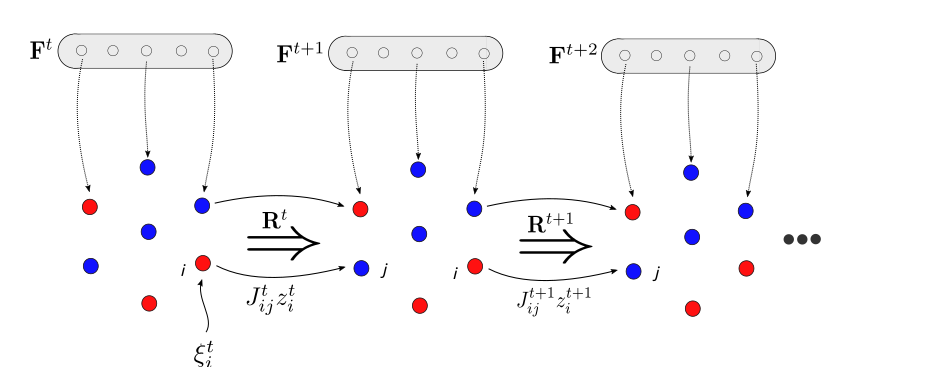
\includegraphics[width=150mm]{figure-1}
\caption{(a) Diagram of a recurrent neural network receving a time-dependent feedforward stimulus. (b) Diagram of the stochastic encoding scheme used a recurrent neural network with noise}
\end{figure}

In addition to non-trivial correlations in their spike timing, neurons in cortical networks tend to exhibit highly irregular time intervals between spikes. The stochasticity in spike timing has can be attributed to cellular and sensory noise (Faisal 2008), or alternatively to network-scale mechanisms such as excitatory-inhibitory balance (Vreeswijk 1996, 1998). Amidst this irregularity, our understanding of spike correlations are further complicated by the nonlinear dynamics of recurrent network models (Baker 2019; Tetzlaff 2008, 2012; Doiron 2016; Ocker 2017). It is common to tame this complexity by making suitable combinations of assumptions regarding the statistics of network stimuli, the mechanism of neuron-neuron interactions, or the statistics of synaptic connectivity. In the mean-field approximation strong assumptions are often made regarding the synaptic connectivity in order to estimate the mean value of synaptic currents. As a rule, the postsynaptic current to a neuron embedded in a spiking network consists of two components: feedforward and feedback (sometimes called recurrent):

\begin{align}
I(t) = F(t) + R(t) + \xi(t)
\end{align}

Notice that an additional noise term $\xi(t)$ to capture channel noise or noise in the synaptic integration process. This is frequently taken to be a i.i.d Gaussian white noise. A variety of models for the integration of this current into a stateful membrane potential exist. Here, we are particularly interested in non-linear integrate and fire models which are described by the Langevin equation

\begin{equation}
\tau\dot{V}(t) = E - V + \psi(V) + I(t)
\end{equation}

where the function $\psi(V)$ is a function of the membrane potential. An important case of (1.2) is the exponential integrate and fire (EIF) model where $\psi(V) = \Delta_{T}\exp\left(\frac{V-V_{T}}{\Delta_{T}}\right)$ is a spike generating current. This model is an extension of the standard linear integrate and fire models which more accurately captures the initial dynamics of opening of spike-generating sodium channels (Richardson 2007). To produce spiking behavior, the membrane potential is passed through a thresholding function which produces spike trains, which are represented as sums over delta functions

\begin{equation}
z_{j}(t) = \sum_{i} \phi(t) * \delta(t-t_{i})
\end{equation}

where the variable $z_{j}(t)$ is sometimes called the \emph{observable state} of neuron $j$ and is given by thresholding the voltage: $z_{j}(t) = H(v_{j}(t) - \theta)$ where $H$ is the Heaviside step function. The time-dependent firing rate of a neuron is given by averaging the above spike train across multiple realizations $r_{j}(t) = \langle z_{j}(t) \rangle$. In addition, to avoid instantaneous synapses, $z_{j}(t)$ is convolved with the synaptic kernel $\phi(t)$, which is often taken to be a decaying exponential, as is done in later sections. Immediately after firing an action potential, the membrane potential is reset to a resting value $V_{\mathrm{reset}}$ and it is held there for a refractory period $\tau_{\mathrm{ref}}$. Importantly, in a recurrent network, (1.3) is directly related to the feedback current in (1.2) by 

\begin{equation}
R_{j}(t) = \sum_{i} J_{ij}(t)\cdot \phi(t) * \delta(t-t_{i})
\end{equation}

Ultimately, an important goal is to understand the origins of correlations or lack thereof in the variable $z_{j}(t)$ across a population of neurons. One mechanism for achieving this is provided by the mean field approximation.

\subsection{The mean-field approximation}

As mentioned, theoretical work has proposed that the irregular inter-spike intervals observed in cortex can be explained by approximate balance of excitatory and inhibitory synaptic currents (Vreeswijk, 1996). In this balanced regime, the timing of the firing of cells in cortex is sensitive to the relatively small fluctuations in their total synaptic input because the excitatory and inhibitory inputs cancel each other (Amit, 1995). Also, excitatory and inhibitory balance has been theoretically shown to enhance the sensitivity of fast stimulus fluctuations much smaller than a typical integration time constant for a single neuron (Vreeswijk, 1996; Tian 2020). Interestingly, model neurons optimally detect temporal information when the average membrane potential is one standard deviation of the noise below threshold, a phenomenon known as stochastic resonance (Plesser, 2000; Kempter, 1998). A general framework for generating balanced networks has been developed. In the following paragraphs, the terminology and mathematical machinery introduced in (Vreeswijk 1996) and later used by (Renart 2010; Rosenbaum 2017) and others will be described.

First, a quick note on terminology. A network model will be called \emph{logically connected} when connection probabilities are not a function of spatial coordinates. Therefore, a network will be called \emph{spatially connected} or \emph{spatially extended} when they are. The networks considered will be primarily logically connected, although spatially extended networks will be explored later (see Results). Furthermore, a network model is called \emph{sparse} if the probability of a connection between a neuron in a population $\alpha$ and another neurons in a population $\beta$ scales with the network size $N$ according to $p_{\alpha\beta} \sim \mathcal{O}(1/N)$. As a result, the degree $K$ of a neuron does not depend on the scale of the network or $K \sim \mathcal{O}(1)$. In contrast, we then say that a network is \emph{dense} if the above connection probability scales as $p_{\alpha\beta} \sim \mathcal{O}(1)$ such that the degree of a neuron scales as $K \sim \mathcal{O}(N)$. Moreover, the efficacy of a synaptic connection between populations $\alpha$ and $\beta$ is said to be \emph{strong} if $J_{\alpha\beta} \sim \mathcal{O}(1)$ and \emph{weak} coupling occurs when $J_{\alpha\beta} \sim \mathcal{O}(1/\sqrt{N})$. This choice of scaling for $J_{\alpha\beta}$ and the degree $K$ results in the total synaptic input to a neuron scaling as $\mathcal{O}(\sqrt{N})$. In this case, it is possible parameterize the network such that fluctuations in the synaptic input currents saturates to a value of the order of the spiking threshold, in the limit of large $N$ (Vreeswijk, 1996; Renart 2010; Rosenbaum 2017).  

The scaling of synaptic inputs outlined above is a critical step towards finding the balanced state. To see this, consider the total synaptic current injected into a neuron $i$ within a population $\alpha$, decomposed into its feedfoward and recurrent components

\begin{align}
I_{i}^{\alpha}(t) &= F_{i}^{\alpha}(t) + R_{i}^{\alpha}(t)\\
&= F_{i}^{\alpha}(t) + \sum_{\beta}\sum_{j} \frac{J_{ij}^{\alpha\beta}}{\sqrt{N}}(\phi * z^{\beta}_{j}(t))
\end{align}

Again, for the sake of generality, the term $z^{\beta}_{j}(t)$ is convolved with a with a synaptic kernel $\phi$, determining the shape of the post-synaptic potential induced by a spike. In the mean-field approximation we replace the current in each term of the sum over $j$ in (1.2) by its average value, which is a valid approximation in the limit $N\rightarrow\infty$ (Vreeswijk 1996). For the sake of simplicity, take $\phi = \delta(t)$, and the observable state $z^{\beta}_{j}(t)$ is replaced by the average firing rate of a neuron in population $\beta$ multiplied by the probability of a connection $p_{\alpha\beta}$

\begin{align*}
\langle I_{i}^{\alpha}(t)\rangle &= \langle F_{i}^{\alpha}(t)\rangle + \langle R_{i}^{\alpha}(t)\rangle\\
&= \langle F_{i}^{\alpha}(t)\rangle + \sqrt{N}\sum_{\beta}j_{\alpha\beta}p_{\alpha\beta}r_{\beta}
\end{align*}

with $j_{\alpha\beta} = J_{\alpha\beta}\sqrt{N}$. Notice that the average value of the recurrent contribution to the synaptic current indeed saturates for large $N$. Writing the above equation explicitly for a neuron in an excitatory-inhibitory network i.e. $\alpha, \beta \in \{e, i\}$

\begin{align}
\langle I_{j}^{e}(t)\rangle &= \langle F_{j}^{e}(t)\rangle + \sqrt{N}\left(j_{ee}p_{ee}r_{e} + j_{ie}p_{ie}r_{i}\right)\\
\langle I_{k}^{i}(t)\rangle &= \langle F_{k}^{i}(t)\rangle + \sqrt{N}\left(j_{ii}p_{ii}r_{i} + j_{ei}p_{ei}r_{e}\right)
\end{align}

If we require that, in the mean-field limit $N\rightarrow\infty$, the average current vanishes and that $\langle F_{j}^{\alpha}(t)\rangle \sim \mathcal{O}(\sqrt{N})$ we have the following matrix equation relating the mean field firing rates to the synaptic weights and average feedforward current

\begin{align}
\begin{pmatrix}
j_{ee} & j_{ie}\\
j_{ei} & j_{ii}
\end{pmatrix}
\begin{pmatrix}
r_{e}\\
r_{i}
\end{pmatrix}
= 
-\begin{pmatrix}
\langle F_{j}^{e}\rangle\\
\langle F_{k}^{i}\rangle
\end{pmatrix}
\end{align}

Assuming that the above matrix is invertible, we have the following solution

\begin{align}
\underset{N\rightarrow \infty}{\mathrm{lim}}r_{e} = \frac{\langle F_{j}^{e}\rangle j_{ii}-\langle F_{k}^{i}\rangle j_{ie}}{j_{ei}j_{ie} - j_{ee}j_{ii}}
\end{align}

\begin{align}
\underset{N\rightarrow \infty}{\mathrm{lim}}r_{i} = \frac{\langle F_{k}^{i}\rangle j_{ee}-\langle F_{j}^{e}\rangle j_{ei}}{j_{ei}j_{ie} - j_{ee}j_{ii}}
\end{align}

For positive solutions for the above firing rates and for the above matrix to be invertible we have the rather loose condition $\langle F_{j}^{e}\rangle/\langle F_{k}^{i}\rangle > j_{ie}/j_{ii} > j_{ee}/j_{ei}$ and we recover the condition given in (Rosenbaum 2014; Rosenbaum 2017; Akil 2021). Notice that the parameters specific to the neuron model do not enter into the equation above. 

The technique used above has also been extended to account for correlations in neural spike trains arising from correlation in synaptic currents. Indeed, this method has been successfully generalized to logically coupled networks with many populations as well as networks which are spatially extended (Rosenbaum 2017). It has also been applied to discrete networks receieving temporally correlated stimuli (Baker 2019). However, proving the existence of a balanced state simultaneously requires some rather harsh assumptions about the synaptic weights. Weight distributions observed in experiments are unimodal and long-tailed (Perin 1997; Song 2005). Also, the method is not readily generalizable to plastic networks, although deviations from the balanced state under a spike-timing dependent plasticity rule have been described (Akil 2021). Nevertheless, the balanced state is a natural starting point for simulations, as it successfully captures the spike-timing irregularity observed \emph{in-vivo}.

\subsection{The diffusion approximation and linear response}


A fundamental approximation used to estimate the dynamics of excitatory-inhibitory networks is the so-called \emph{diffusion approximation}. If the presynaptic partners of a neuron are described by an inhomogeneous point process, the total synaptic current $I(t)$ can have complex statistics depending on presynaptic firing rates and their correlations. However, in some special cases, such as when presynaptic firing rates are large, synaptic currents are safely assumed to be Gaussian (Richardson 2007). To begin to examine this, we combine equations (1.1), (1.2), and (1.4) for a single neuron $i$ to give 

\begin{equation}
\tau\dot{V}_{i}(t) = E_{i} - V_{i} + \psi(V_{i}) + F_{i}(t) + \xi(t) + \sum_{j} J_{ij}(t)\cdot \left(\phi(t) * z_{j}(t)\right)
\end{equation}

where it is implicitly assumed that $\xi(t)$ is a delta correlated white noise i.e. $\langle\xi_{i}(t)\xi_{j}(t)\rangle = \delta_{ij}$ and $\langle\xi_{i}(t)\xi_{i}(t')\rangle = \delta(t-t')$. When expressed for all neurons $i$ simultaneously, the above becomes a high-dimensional stochastic differential equation, which in general is difficult to work with. Previously, a realization of the spike train $z_{i}(t)$ that arise from thresholding (1.12) are approximated as a sum of two terms which represent the spike train in the absence of feedforward and feedback currents and a linear filter of synaptic inputs

\begin{align}
z(t) \approx z_{0}(t) + (A * X)(t) 
\end{align}

If averaged over many realizations, the above instead becomes an expression for the firing rate $r(t)$. The equation above is the central claim made by a linear reponse theory of network dynamics. For simplicity, it is natural to start with the case where $F_{i}(t)$ is itself a Gaussian white noise independent of the intrinsic noise. Therefore, the intrinsic noise $\xi(t)$ and the feedforward stimulus can be absorbed into a single noise term. Then, $z_{0}(t)$ is a realization of a spike train in the absence of feedback when its stimulation is a sum of feedforward and intrinsic noise. In the frequency domain this equation reads (Linder 2005; Trousdale 2012)

\begin{align}
\tilde{z}_{i}(\omega) = \tilde{z}_{i}^{0}(\omega) + \tilde{A}(\omega)\left(\sum_{j}\tilde{J}_{ij}(\omega)\tilde{z}_{j}(\omega)\right)
\end{align}

The matrix $\tilde{J}(\omega)$ is the frequency domain representation of the synaptic connectivity matrix after convolution with the synaptic kernel and $\tilde{A}(\omega)$ is the transfer function or response function in the frequency domain. This equation can then be rewritten in matrix form to give the frequenty domain representation of the spiking activity across all neurons in the population simultaneously

\begin{align}
\tilde{z}(\omega) = \tilde{z}^{0}(\omega) + \tilde{A}(\omega)\tilde{J}(\omega)\tilde{z}(\omega)
\end{align}

The result above can then be solved for $\tilde{z}(\omega)$ to give 


\begin{align}
\tilde{z}(\omega) = \left(I-\tilde{A}(\omega)\tilde{J}(\omega)\right)\tilde{z}^{0}(\omega)
\end{align}

where $I$ is the identity matrix. The expression above can then be used to obtain the cross-spectrum (and therefore the cross-correlations) of two spike trains $z_{i}(\omega)$ and $z_{j}(\omega)$ for all possible pairs. 

\begin{align}
\langle\tilde{z}(\omega)\tilde{z}^{*}(\omega)\rangle &= \langle \left(I-\tilde{A}(\omega)\tilde{J}(\omega)\right)\tilde{z}_{0}(\omega)\tilde{z}_{0}^{*}(\omega)\left(I-\tilde{A}(\omega)\tilde{J}(\omega)\right)^{*}\rangle\\
&= \Delta(\omega)C^{0}(\omega)\Delta(\omega)^{*}
\end{align}

The above result is the matrix of cross spectra across the population $C(\omega)$ in the situation where feedforward inputs are uncorrelated.
In essence, a linear response theory of network dynamics determines the auto- and cross-correlations of spike trains. Studies have used the above result as a foundation for analyzing the effects of the topology $J$ on the matrix $C(\omega)$ (Trousdale 2012; Ocker 2015). In any case, the matrix $C^{0}(\omega)$ and the linear response function $A(\omega)$ are still unknown, and must be found. In general, this can be challenging; however, the assumption that feedforward inputs and intrinsic noise are white permits the use of the diffusion approximation. In other words, we can use the Fokker-Planck equation to estimate $C^{0}(\omega)$ and $A(\omega)$ by using methods introduced in (Richardson 2007). The primary result of that study is a numerical solution to the Fokker-Planck equation under a weak sinusoidal perturbation to the synaptic current (Richardson 2007; 2009). 

Under conditions in which the diffusion approximation applies, the Kramers-Moyal expansion can be reduced to the following Fokker-Planck equation for the general nonlinear stochastic integrate and fire model given in (1.4)

\begin{align}
\frac{\partial P(V,t)}{\partial t} &= \frac{\sigma^{2}}{2}\frac{\partial^{2}P}{\partial V^{2}} + \frac{\partial}{\partial V}\left(\frac{V-E-\psi}{\tau}P\right)
\end{align}

The stationary solution of the density $P(V,t)$ has been found for simple models such as when $\psi(V) = -V$, which resembles the Ornstein-Uhlenbeck process with special boundary conditions imposed by the threshold (Brunel 2000; Brunel and Hakim 1999). However, the solution for non-linear integrate and fire models frequently requires numerical integration of (1.5) to find the stationary density over the membrane potential and to estimate steady state firing rates. If (1.13) is resolved into a pair of first order differential equations, we have

\begin{align*}
\frac{\partial P(V,t)}{\partial t} &= -\frac{\partial J}{\partial V}\\
J &= \frac{E-V+\psi}{\tau} - \frac{\sigma^{2}}{\tau}\frac{\partial}{\partial V}
\end{align*}

Details of the numerical integration (sometimes called the threshold integration method) of the above pair of equations are known for stationary white noise input. See (Richardson 2007; 2009) for a full derivation of these methods. The first step is to compute the stationary density for the membrane potential by solving the Fokker-Planck equation under white-noise stimulation. This simultaneously provides the steady state firing rate $r_{0}$. The steady state firing rate can then be used to derive the frequency spectrum $C^{0}(\omega)$. Once this is obtained, the frequency response can be found by using Richardson's method of solving the Fokker-Planck equation for a weak sinusoidal perturbation in the synaptic current.It should be noted that the diffusion approximation is not limited to this context. Rather, it also applies when synaptic connectivity is sufficiently sparse, and the probability of two neurons sharing synaptic inputs vanishes. Then, the synaptic current to a neuron can be guaranteed to follow a normal distribution, per the central limit theorem (Brunel 2000). However, the diffusion approximation is not exclusive to these network architectures either. It is also a valid assumption when the population fires asychronously and the feedback $R(t)$ is a sum over independent processes, even in dense networks (Tian 2020; Rosenbaum 2017).

Furthermore, the solution for $C(\omega)$ given in (1.2) has been derived in an alternative fashion by using an iterative approach (Trousdale 2012). This approach is highly valuable as it builds an estimate of $C(\omega)$ by considering paths through a recurrent network of increasing length. However, the mathematics used to derive an estimate of $C(\omega)$ is very dense. Here, only the key points will be highlighted and most of the mathematical details are deferred to the original text (Trousdale 2012). Intuitively, the spike-train correlation between a pair of cells can be estimated from the activity of presynaptic cells $n$ synapses away from the cells under consideration. We expect then to improve our estimate of $C(\omega)$ for large values of $n$. For the simplest case, when $n=0$, the neurons are uncoupled and we have $C(\omega) = C^{0}(\omega)$. Now, when $n=1$, we consider only the nearest neighbors in calculating the cross-correlation between neurons $i$ and $j$ and improve on the estimate $C^{0}(\omega)$ by computing

\begin{align}
z_{i}^{1}(t) = z_{i}^{0} + \sum_{j}K_{ij}[y_{j}^{0}-r_{j}](t)
\end{align} 

As mentioned, the iteration can proceed by incrementing $n$ to account for directed chains with increasing length. If the iteration does proceed to order $n$, then we have a more general form of the above equation (Trousdale 2012)

\begin{align}
z_{i}^{n+1}(t) &= z_{i}^{0} + K*[z^{n}-r](t)\\
&= z_{i}^{0} + \sum_{k=1}^{n+1} K^{(k)} *[z^{0}-r](t)
\end{align} 

As in the original derivation, $K^{(k)}$ is the k-fold convolution of $K$ with itself. A central result of (Trousdale 2012) was the following expression for the $n$-th order estimate of the matrix $C(\tau)$ 

\begin{align}
C^{n}(\tau) = \sum_{m}\sum_{n} K^{m}*C^{0}*(K^{n})^{T}(\tau)
\end{align} 

After taking the Fourier transformation and the limit $n\rightarrow\infty$ gives a result identical to (1.18). Most importantly for this thesis, this method been extended to also account for the network response to external signals. In this case, the estimate of $z(t)$ up to a chain of length $n$ gives

\begin{align}
z^{n+1}(t) &= z^{0} + K*[z^{n}-r](t) + A*F(t)
\end{align} 

where $F(t)$ is the feedforward input as usual and $A$ is a diagonal matrix containing the linear response of each neuron in the time domain. In this case, the expression analagous to (1.23) is 

\begin{align}
C^{n}(\tau) = \sum_{m}\sum_{n} K^{m}*C^{0}*(K^{n})^{T}(\tau) + \sum_{m}\sum_{n} K^{m}*A*C^{ext}A(K^{n})^{T}(\tau)
\end{align} 

where $C^{ext} = \langle F(t+\tau)F(t)^{T}\rangle$ for $F(t) = [F_{1}(t)\;,...,\;F_{N}]$ (the cross-correlation matrix of the external signals). Transforming (1.25) to the frequency domain as before then gives a crucial result (Trousdale 2012; Ocker 2017). 


\begin{align}
C(\omega) &= \Delta(\omega)\;C^{0}\;\Delta^{*}(\omega) + \Delta(\omega)\;A(\omega)C^{\mathrm{ext}}(\omega)A^{*}(\omega)\;\Delta^{*}(\omega)
\end{align} 

Here, we are particularly interested in using (1.26) to estimate the matrix $C(\omega)$ when the feedforward inputs $F(t)$ are drawn from a multivariate gaussian distribution i.e. $F(t) \sim \mathcal{N}(\mu,\Sigma)$. This can be done; however, it has been noted that corrections for $C^{0}(\omega)$ are needed. These corrections are detailed in the methods section of (Trousdale 2012).

In summary, the linear theory provides a direct mechanism for solving for the cross-covariance of spiking in the population in terms of the synaptic coupling matrix, for arbitrary network topologies. Previous analyses have restricted feedforward inputs to be uncorrelated (Trousdale 2012; Ocker 2015). Other analyses have considered more complex network topologies with a spike-timing dependent plasticity rule, but still have left external input uncorrelated (Ocker 2015). A natural development is to then generalize these approaches to the case where the network topology can be dynamic and the feedforward inputs have nonzero correlations.


\subsection{Reshaping network structure with synaptic plasticity}

Activity dependent modification of synaptic efficacy or the formation of new synapses is the putative basis of learning and memory formation. In his famous neurophysiological postulate, Donald Hebb suggested that repeated stimulation of specific receptors of sensory signals would lead to the formation of a \emph{cell assembly} and these structural changes would constitute a representation or imprint of an internally or externally generated sensation (Hebb 1949). The chaining of these assemblies then could provide a structural basis for cognitive processes such as memory retrieval, reasoning, and planning (Buzaki 2010). Recent neurobiological advances have provided substantial insight on the biochemical and biophysical mechanisms of plasticity. However, the formation of functional circuits and their stability amidst ongoing network dynamics remains unclear.

Plasticity mechanisms are highly diverse and occur over a wide range of time scales: from milliseconds to hours to days (Zenke 2015). For example, short-term synaptic plasticity (STP) is thought to provide a richer set of network responses to stimuli without permanently altering the circuit architecture. One of several mechanisms thought to underly STP can be seen by the repeated stimulation of a presynaptic cell causing a transient accumulation of calcium in the presynaptic terminal, which has been proposed as a mechanism for short-term memory (Mongillo 2008). Calcium ions elevate the probability of neurotransmitter release due to its proposed interaction with the biochemical machinery involved in synaptic vesicle excytosis. Other short term changes in synaptic efficacy can occur such as the facilitation or depression based upon the temporal characteristics of the stimulus. Paired-pulse experiments have yielded evidence that tetanic stimulation can result in inactivation of voltage-dependent sodium and/or calcium channels or depletion of the release ready pool of synaptic vesicles at the presynaptic terminal. Synaptic efficacy can alternatively be lowered by the release of biochemical neuromodulators which can interact with the synaptic machinery to inhibit the release of neurotransmitter into the synaptic cleft. Thus, these neuromodulators can also play a role in facilitation or depression in STP.

It is well-accepted that neural circuits also possess the mechanisms for long term changes in synaptic strength formally referred to as long term potentiation (LTP) and long term depression (LTD). The brain encodes internally and externally generated stimuli as spatiotemporal patterns of action potentials and long-term modifications to such patterns via changes in synaptic transmission provide a feasible mechanism for the storage of information. In other words, permanent or semi-permanent changes in synaptic weights alter the spatiotemporal response of population of neurons to stimuli and therefore provide a method for long term memory formation. Since its inception by Cajal, this idea has been rigorously tested, for example in the CA1 region of the hippocampus (Whitlock et al. 2006). The modification of spatiotemporal characteristics of the neural response to stimuli suggest that evidence for plasticity can be found in the correlation structure of neural spike trains.

Early work on synaptic plasticity at the cellular level demonstrated that LTP in slices of hippocampal tissue could occur as a result of tetanic (high-frequency) stimulation of a post-synaptic cell (Bliss 1973) while low frequency stimulation can drive LTD. If many fibers are stimulated at frequencies exceeding $50\text{Hz}$, postsynaptic potentials can increase by 50-100\% (Sejnowski 1989). Additional research expanded upon this observation, noting that temporal correlation of presynaptic and postsynaptic spiking affected plasticity. In particular, strong temporal correlation on a timescale of $\pm 100 \text{ms}$ gave rise to LTP while weak correlations LTD. These phenomenological studies of plasticity have resulted in a number of different plasticity rules which fall under the umbrella of `Hebbian' learning rules. Hebbian learning rules have been broadly defined as rules in which the change in synaptic efficacy depends only on pre-synaptic and post-synaptic variables and that updates to the weight depends interactively on these two variables and not separately (Sejnowski 1989).  Additionally, Hebbian learning rules are \emph{causal} in that LTP occurs when the presynaptic neuron contributes to the firing of the postsynapic cell and LTD occurs otherwise.

Additional efforts demonstrated that the sign and magnitude of LTP and LTD dependend on the order and delay of presynaptic and postsynaptic action potentials, on a time scale of $10\text{ms}$ (Markram 1997), later named spike timing dependent plasticity (STDP) (Song 2000). In the original formulation of Hebbian STDP, LTP can occur when presynaptic spikes lead postsynaptic spikes by $\sim 20\mathrm{ms}$ and LTD can occur when postsynaptic spikes lead presynaptic spikes by $\sim 20-100\mathrm{ms}$ (Markram 1997; Bi and Poo 1998; Celikel 2004; Feldman 2012). However, plasticity does not only depend on spike timing, but also on other factors such as firing rates, and synaptic cooperativity, and postsynaptic voltage (Makram 1997; Sjosstrom 2001; Feldman 2012). Therefore, findings indicate that STDP is part of a broader class of plasticity rules and may be viewed as the spike timing component of a multifactor plasticity rule (Feldman 2012).

Furthermore, the biochemical mechanism of synaptic plasticity is regulated by the release of neurotransmitters by the presynaptic cell and/or by modifying the density of receptors at the postsynpatic membran (Sumi 2020). Indeed, it is widely believed that presynaptic release of glutamate results in activation of $\alpha$-amino-3-hydroxy-5-methyl4-isoxazolepropionic acid receptor (AMPAR) and subsequent depolarization of the post-synaptic membrane. Membrane depolarization then activates the N-methyl-D-aspartate receptor (NMDAR), which is permeable to Ca2+ - a prefactor for a biochemical cascade resulting partially in the trafficking of AMPA receptors to the postsynaptic membrane. High elevations in Ca2+ concentrations in the presynaptic cell are believed to result in an increased density of AMPA receptors at the postsynaptic membrane and in elevated excitatory postsynaptic potentials (EPSPs) thereby providing a mechanism for LTP (Sumi 2020). In summary, LTP versus LTD inducation is determined by the magnitude and time course of calcium flux (Lisman 1989; Yang 1999; Feldman 2012). When the presynaptic cell fires first, the EPSP produces a strong NMDAR calcium flux while while when the postsynaptic cell fires first, this flux is weak. On the other hand, LTD has not been shown to occur soley due to minor elevations in Ca2+ concentrations, but is thought to result from a retrograde signaling mechanism in which presynaptic transmitter release probability is decreased (Nabavi 2013).

Beyond spike-timing dependent plasticity, other plasticity mechanisms have been observed experimentally. In the hippocampus, non-Hebbian heterosynaptic LTD alongside LTP was described shortly after the phenomenon of LTP was discovered (Lynch 1977). The Hebbian mechanisms or \emph{associative mechanisms} discussed above are termed homosynaptic mechanisms, as they depend on both pre- and post-synaptic activity. There are also heterosynaptic mechanisms which depend on only the state of the post-synaptic neuron and are thought to exist to counteract chaotic dynamics introduced by Hebbian-type rules and to balance synaptic changes (Chistakova 2014). Hebbian homosynaptic learning rules, by definition, potentiate (depress) synapses with positive feedback, meaning that increasing (decreasing) synaptic efficacy will promote further potentiation (depression). For example, The standard doublet STDP model gives rise to splitting of synaptic weights, producing a bimodal distribution; however, weight distributions observed in experiments are unimodal and long-tailed (Perin 1997; Song 2005). The result is the overexcitability of some neurons and silencing of others making network dynamics unstable. Induction of LTD at high firing rates of the postsynaptic neuron is a candidate for an intrinsic stabilization mechanism (Kempter 2001). Also, it has been recent suggested that rate-dependent terms in the synaptic learning rule can stabilize motif configurations (Ocker 2015). Ultimately, it is thought that a push-pull mechanism exists in which homosynaptic LTP prevents the network from falling silent at low firing rates while heterosynaptic LTD prevents the runaway dynamics at high firing rates.

Understanding the stable formation and maintenance of cell assemblies is an additional goal of synaptic plasticity research. From a naive point of view, a cell assembly could form if a subset of a neuron's inputs were to potentiate while other inputs depress. However, for this to occur both groups should be repeatedly activated either with highly specific patterns to promote LTP or LTD, respectively (Chistikova 2014). This would then limit network stability to special sequences of input patterns while we expect that plasticity mechanisms exist to promote stability under a variety of input stimuli. Moreover, experiments involving intercalated neurons of the amygdala have demonstrated that LTP induction with high-frequency stimulation can simultaneously result in heterosynaptic depression (Royan 2003). Conversely, LTD induction with low-frequency stimulation was also shown to induce LTP. These observations indicate the existence of intracellular signaling that would provide synapses with `awareness' of eachother. Learning rules which depend on the post-synaptic firing rate would produce a similar result, although often these rules do not perform selective potentiation or depression. That is, synaptic weights are normalized without regard to which synapses can be blamed for chaotic or silent neuron states. In circuits with highly regular organization of the inputs, such as the hippocampus or amygdala, the onset of LTP can induce weaker LTP at nearby inputs while concurrently inducing heterosynaptic LTD at more distant inputs, while the magnitude of LTD decreasies with distance (Royer 2003; White 1990).

The experiemental observations discussed suggest that balanced LTP and LTD may be a powerful mechanism of for synaptic normalization and synaptic competition. Thus, several computational studies incorporating more realistic forms of synaptic plasticity with conductance based neuron models have surfaced e.g., (Zenke 2015; Kumar 2014). Many have incorporated a balance between excitation and inhibition to capture the irregular activity of cortical networks, but stable formation of cell assemblies is difficult to achieve. This shortcoming could, in part, be due to the tendency of STDP to lead to pathological behavior in balanced networks (Morrison 2007). The introduction of homeostatic mechanisms such as normalization of total excitatory conductance alongside inhibitory STDP to control the firing rate of excitatory neurons has been used to inhibit pathological activity in the balanced regime (Kumar 2014). At the same time, the spatial properties of homeostatic plasticity mechanisms mentioned above have yet to be investigated. This, in combination with spatially dependent connection probabilities as in (Rosenbaum 2017) could provide insight into the stabiliy of cell assemblies.

In plastic networks, synaptic weights (conductances) are functions of time, thus we expand $I(t)$ as a sum of individual conductances as in (Zenke 2015) to give a total current for a single neuron

\begin{align*}
I_{j}^{\alpha}(t) &= \sum_{\beta}\sum_{i} g_{ij}^{\beta}(t)(E_{\beta} - V_{j})\\
&= \sum_{\beta}\sum_{i}J_{ij}^{\alpha\beta}(t)\left(\phi\;*\;z_{i}(t)\right)(E_{\beta} - V_{j})
\end{align*}

where $\alpha \in \{E,I,X\}$. To be clear, excitatory conductances, whether in the external or primary population would be under the control of an inhibitory neurotransmitter such as gamma-aminobutyric acid (GABA) while inhibitory conductances would be under the control of glutamate e.g., AMPAR/NMDAR. Notice that the time-dependence of $g^{\alpha}$ can then be given by the convolution of an excitatory presynaptic spike train $z_{i}(t)$ or inhibitory spike train $z_{k}(t)$ with an appropriate synaptic kernel $\phi$. The synaptic plasticity rule is then a rule for the time-derivative $\dot{J}^{\alpha\beta}_{ij}$.

\begin{figure}[t!]
\centering
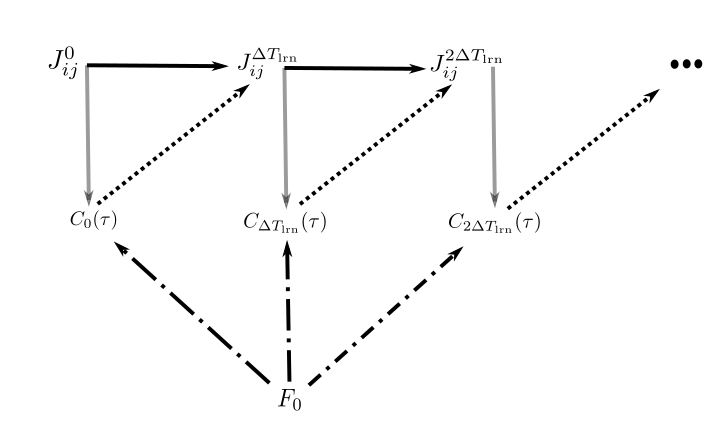
\includegraphics[width=130mm]{figure-6}
\caption{Computational graph describing the update of synaptic weights $J_{ij}$ and the cross-covariance matrix $C(\tau)$ over multiple stimulus periods of length $\Delta T_{\mathrm{stim}}$. The learning period $\Delta T_{\mathrm{lrn}}<< T_{\mathrm{stim}}$ determines the frequency of learning updates within the period $\Delta T_{\mathrm{stim}}$}
\end{figure}

The cellular machinery of plasticity mechanisms described above highlights the importance of spike-time correlations, generated by recurrent feedback or feedforward projections, in determining the evolution of synaptic weights. A classic derivation of the evolution of synaptic weights for interacting Poisson processes was given by Kempter et al. (Kempter 1999). This result is an important starting point for later analysis. Consider the total change in the synaptic weight between neurons $i$ and $j$ as $\Delta J_{ij} = J_{ij}(t+\Delta t) - J_{ij}(t)$ in a time interval $\Delta t$. Consider the very general rule for a single spiking neuron $i$ receiving many inputs $1 < j \leq N$ 
\begin{align*}
\dot{J_{ij}} = a_{0} + a_{i}z_{i}(t) + a_{j}z_{j}(t) + F(z_{i}(t),z_{j}(t))
\end{align*}

for a yet unknown function $F$, which could be a STDP rule, for example. We will assume that the constant growth or decay term $a_{0}$ is zero. Spike trains are a summation of delta functions over time, i.e. $z_{i}(t) = \sum_{n} \delta(t-t_{i}^{n})$ and $z_{j}(t) = \sum_{m} = \delta(t-t_{j}^{m})$. If we consider only rules that consider the timing of pairs of spikes, changes in synaptic weight can occur from the arrival of a presynaptic spike $z_{i}(t) = 1$, a postsynaptic spike $z_{j}(t) = 1$ or as a function of the delay in spike timing  $\tau = t_{i}^{n} - t_{j}^{m}$. The spike-timing component of the learning rule is given by the learning window function $W(t_{i}^{n} - t_{j}^{m})$. Integrating over a time window $\Delta T_{\mathrm{lrn}}$ gives the total change $\Delta J_{ij}$ (Kempter 1999)


\begin{align}
\Delta J_{ij}(\Delta T_{\mathrm{lrn}}) &= \int_{0}^{\Delta T_{\mathrm{lrn}}} dt'\left(a_{i}z_{i}(t') + a_{j}z_{j}(t')\right) \\
&+ \int_{0}^{\Delta T_{\mathrm{lrn}}} dt'\int_{0}^{\Delta T_{\mathrm{lrn}}} dt''W(\tau)z_{i}(t'')z_{j}(t')
\end{align}

The stochasticity of the spike functions $z_{i}(t)$ and $z_{j}(t)$ means that we can only hope to derive the behavior of the above integral on average. In other words, $\Delta J_{ij}$ is itself a stochastic process but we can focus on its drift or expected rate of change. Simulaneously, $z_{i}(t)$ and $z_{j}(t)$ are strongly dependent on the weights $J_{ij}$; however, if the time scale of plasticity $\Delta T_{\mathrm{lrn}}$ is sufficiently long compared to the correlation time scale of the neurons activity, the correlation between $z_{i}(t)$ and $z_{j}(t)$ can be treated as stationary (Kempter 2001). Importantly, the effective correlation time scale of neuron dynamics is intimately related to the timescale over which it is `picked up' by the learning window $W(\tau)$. Analyzing the drift in $\Delta J_{ij}$ then reads


\begin{align*}
\Delta T_{\mathrm{lrn}}\frac{\langle \Delta J_{ij}\rangle(t)}{\Delta T_{\mathrm{lrn}}} &= \int_{0}^{\Delta T_{\mathrm{lrn}}} dt'\left(a_{i}z_{i}(t') + a_{j}z_{j}(t')\right)\\
&+ \int_{0}^{\Delta T_{\mathrm{lrn}}} dt'\int_{-t'}^{\Delta T_{\mathrm{lrn}}-t'} d\tau W(\tau)\langle z_{i}(t'+\tau)z_{j}(t')\rangle\\
\end{align*}

Note that we can make the same approximations for a sufficiently slow process as we can for a relatively fast process with high time resolution. Then, if synaptic plasticity is sufficiently slow, then we can approximate the average rate of change as $dJ_{ij}/dt \approx \Delta J_{ij}/\Delta T_{\mathrm{lrn}}$, and the bounds of integration can be set to $-\infty$ and $+\infty$ (Kempter 1999) and we have the final result


\begin{align}
\Delta T_{\mathrm{lrn}}\frac{d J_{ij}(t)}{dt} &=  a_{i}\langle z_{i}(t)\rangle  + a_{j}\langle z_{j}(t)\rangle + \int_{-\infty}^{+\infty} d\tau W(\tau)C_{ij}(\tau)
\end{align}

where $\langle z_{i}(t)\rangle$ and $\langle z_{j}(t)\rangle$ can be interpreted as the instantaneous firing rate of neurons $i$ and $j$, respectively. It has already been shown that linear response theory can be used to estimate $C_{ij}(\tau)$ for arbitrary network topologies (Pernice 2012). Furthermore, the equation (1.22) including the instantaneous post-synaptic firing rate can serve as a homeostatic term if $a_{j} < 0$. Although, as highlighted previously, rate-dependent terms in the learning rule do not selectively enforce LTP and LTD since the term $a_{j}\langle z_{j}(t)\rangle$ appears in the equation for $\dot{J_{ij}}$ for all input neurons $i$ (assuming $a_{j}$ is a constant). Thus we need to modify (1.22) to arrive at a synaptic plasticity rule which delivers potentiation or depression heterogeneously, for example using information regarding spatial proximity. Interestingly, a class of spatially connected networks has been studied (Rosenbaum 2011, 2017).



\begin{figure}[t!]
\centering
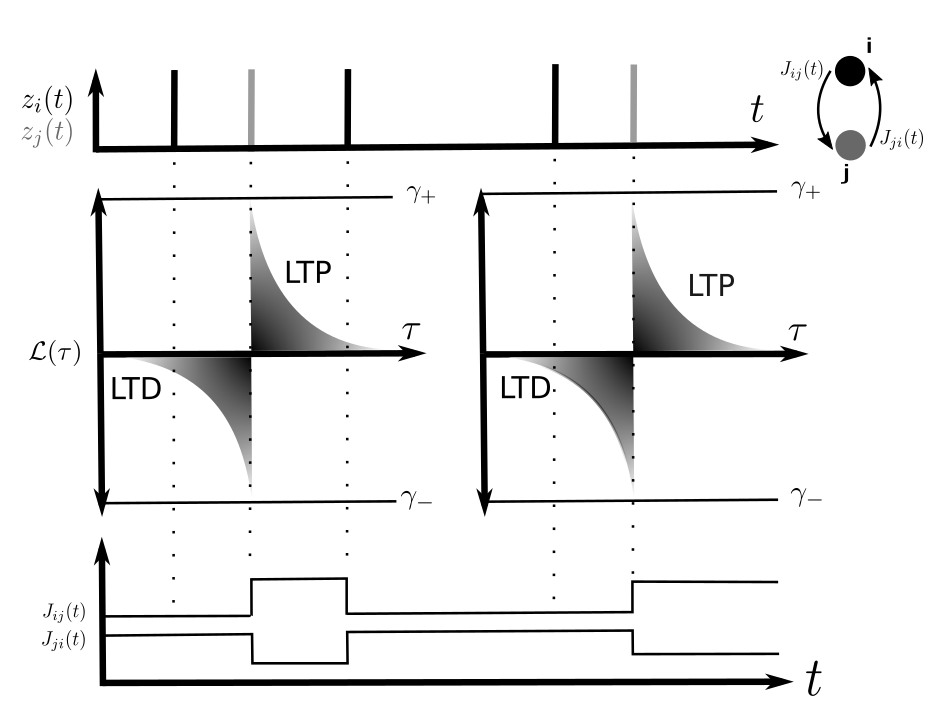
\includegraphics[width=150mm]{figure-2}
\caption{Computational graph describing the update of synaptic weights $J_{ij}$ and the cross-covariance matrix $C(\tau)$ over multiple stimulus blocks of length $\Delta T_{\mathrm{stim}}$. The learning period $\Delta T_{\mathrm{lrn}}<< T_{\mathrm{stim}}$ determines the frequency of learning updates within the period $\Delta T_{\mathrm{stim}}$}
\end{figure}

Say we have the learning window function $W(\tau)$ corresponding to the standard doublet spike-timing dependent plasticity rule

\begin{align*}
W(\tau) = \begin{cases}
      H(J_{max}-J_{ij})\gamma_{+}\exp(-\tau/\tau_{+}), & \text{if}\ \Delta t \geq 0 \\
       H(J_{ij})(-\gamma_{-})\exp(-\tau/\tau_{-}), & \text{if} \;\Delta t < 0
    \end{cases}
\end{align*}

\subsection{Biologically-realistic network topologies}

\begin{figure}[t!]
\centering
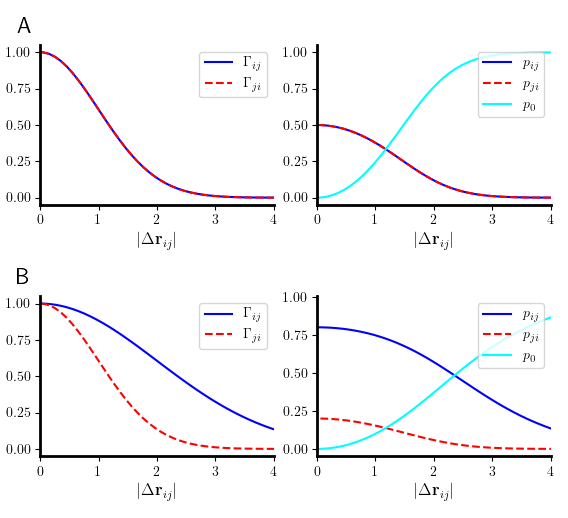
\includegraphics[width=100mm]{figure-7}
\caption{\textbf{Synapse probabilities for gaussian connectivity} (a) Binomial probabilities for two identical gaussian kernels ($\sigma=1$) separated by a distance $|\Delta\mathbf{r}_{ij}|$ and the probability of no synapse $\Gamma_{0}$ (left) and the corresponding multinomial probabilities (right). (b) Binomial probabilities for two different gaussian kernels ($\sigma_{1}=1, \sigma_{2}=2$) separated by a distance $|\Delta\mathbf{r}_{ij}|$ and the probability of no synapse $\Gamma_{0}$ (left) and the corresponding multinomial probabilities (right). }
\end{figure}


Thus far we have considered only the case where the spatial connectivity kernel is the same for every neuron. However, the integrative properties of neurons depend strongly on the number, proportions and distribution of excitatory and inhibitory synaptic inputs they receive (Megias 2001). Also, the role excitatory-inhibitory balance in network dynamics has been a subject of recent debate. Indeed, balanced recurrent excitation and inhibition capture the irregular and asynchronous spiking activity with weak correlations reported in cortex. The spatial extent of excitation relative to inhibition has been shown to have a strong impact on network dynamics. In particular, when the spatial extent of excitation is sufficiently smaller than inhibition, the balanced fixed point loses stability (Rosenbaum 2014). 

To account for excitatory and inhibitory cell types within this framework, we must differentiate $\langle N_{ij}\rangle$ for excitatory and inhibitory neurons and solving for both the mean in-degree and out-degree separately. Thus we have the quantities $\langle E_{E}^{\mathrm{out}} \rangle,\langle E_{I}^{\mathrm{out}} \rangle,\langle E_{I}^{\mathrm{in}} \rangle$ and $\langle I_{E}^{\mathrm{out}} \rangle,\langle I_{I}^{\mathrm{out}} \rangle,\langle I_{E}^{\mathrm{in}} \rangle$. Under the assumption that excitatory and inhibitory neurons are distributed uniformly  in two-dimensional space, we have that $\langle E_{I}^{\mathrm{out}} \rangle = \langle I_{E}^{\mathrm{in}} \rangle$ and $\langle E_{I}^{\mathrm{in}} \rangle = \langle I_{E}^{\mathrm{out}}\rangle$. For brevity, we drop the superscripts and compute the above averages according the general prescription provided by (3.3). The result of these numerical calculations allow us to observe that, for $\Gamma_{0} = 0.2$, the fraction of the target population saturated by excitatory or inhibitory outputs increases monotonically with $\sigma_{E}$ and $\sigma_{I}$  (Fig 3.4 b,d). The parameter maps provided in (Fig 3.4 b,d) are a starting point for our later discussions of newtork dynamics.



\subsection{Prevalent interpretations of network dynamics}

Early theoretical models of neural networks frequently made reference to concepts born in the theory of dynamical systems. Sensory processing was often interpreted as an attraction of the neural state variables to a steady state corresponding to the encoding of the sensory stimulus. This point of view adopts the notion that sensory stimuli are then represented in the brain by \emph{attractor states} or locations in phase space which the network is driven towards during sensory processing (Hopfield, 1982). On the other hand, recent experimental evidence suggests that neurons, synapses, and neural systems are inherently stochastic (Buesing 2011). These observations have provoked a dramatic paradigm shift in the way we view computations as being carried out in the brain. Namely, researchers now widely believe that in some cases information processing by the brain  can be interpreted as a form of probabilistic inference.

Variability in sensory stimuli and the biological constitution of networks of neurons require the brain to make inferences about the external world amidst uncertainty. For example, the perception of objects in the external world by an organism is, in part, the transformation of a noisy continously valued variable to a discrete mental representation of the object. The injection of stochasticity into the pathway mapping stimuli to their neural representation has led many to believe that networks of neurons represent probability distributions rather than implementing logical circuits. Interestingly, behavioral studies have confirmed that human observers not only take uncertainty into account in a wide variety of tasks, but do so in a way that is nearly optimal (Ma 2006). It stands to reason that variability in sensory stimuli and performing inference amidst uncertainty are two sides of the same coin. If sensory stimuli were not variable, meaning that the mapping of sensory stimuli to neural responses was deterministic, the neural response from trial to trial would be identical. Therefore, the ability to handle small variations in the stimulus and the ability to generalize would be diminished.

A typical inference scenario is the deduction of the probability that the observed information was drawn from a distribution already known by the model. That is, the encoding scheme during sensory processing is the distribution of responses conditioned on the stimulus i.e., the posterior distribution $P(R|S)$. In the context of biological and artificial neural networks, that distribution is often \emph{learned} by the model via previous exposure to a large number of samples from the so-called population distribution of the data or stimulus. A popular point of view is that neural activity can be expressed in discrete-time and the set of spikes in each time bin can be interpreted as samples from the posterior $P(R|S)$, a distribution which is encoded by the synaptic weights. This interpretation has spawned the development of interesting parallels between neural dynamics and statistical sampling processes such as Markov chain Monte Carlo (MCMC) sampling (Buesing 2011). However, the interpretation of neural dynamics as implementing an artificial sampling process as in the Boltzmann machine, necessarily excludes biological details, such as synaptic plasticity and spike-adaptation, which are thought to play a major role in neural computation.


\section{Results}

\subsection{Theory}

Introduce a plasticity rule which is a function of space and time

\subsection{Demonstration of the balanced state}




\begin{sidewaysfigure}
\centering

\includegraphics[width=225mm]{figure-3}
\caption{}
\end{sidewaysfigure}

\begin{figure}[t!]
\centering
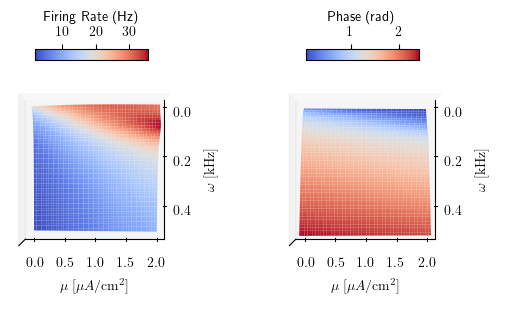
\includegraphics[width=140mm]{figure-4}
\caption{}
\end{figure}

\begin{figure}[t!]
\centering
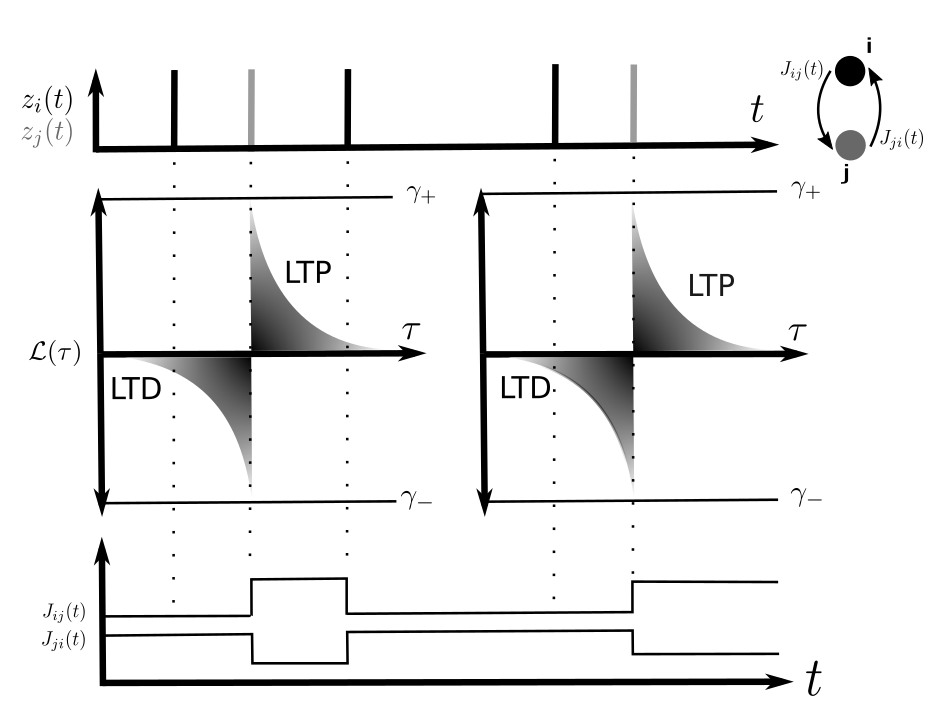
\includegraphics[width=140mm]{figure-5}
\caption{}
\end{figure}


\subsection{The two-dimensional Gaussian network}

Suppose that we have a two-dimensional lattice which contains points separated by a distance $\Delta$ along the axial directions with periodic boundary conditions. The distance between any two points on such a lattice is the following Euclidean distance metric

\begin{align*}
|\Delta\mathbf{r}_{ij}|^{2} = \mathrm{min}(|x_1 - x_2|, n\Delta - |x_1 - x_2|)^2 + \mathrm{min}(|y_1 - y_2|, n\Delta - |y_1 - y_2|)^2
\end{align*}

Now, let the kernel $\Gamma_{ij}$ be the two-dimensional symmetric Gaussian

\begin{align}
\Gamma_{ij}(|\Delta\mathbf{r}_{ij}|) = \gamma\cdot \exp\left(-\frac{1}{2}(\mathbf{r}_{i}-\mathbf{r}_{j})^{T}\mathbf{\Sigma}_{i}(\mathbf{r}_{i}-\mathbf{r}_{j})\right)
\end{align}

where $\mathbf{\Sigma}_{i} = \sigma_{i}^{2}I$ with the two-dimesional identity matrix $I$. The parameter $\sigma_{i}$ can be intepreted as the \emph{reach} of a neuron $i$. Furthermore, for the kernel $\Gamma_{ij}$ to represent a binomial probability at each point of its domain, we must have that


\begin{equation}
\Gamma_{ij}(|\Delta\mathbf{r}_{ij}|)  \leq 1
\end{equation}

Plugging in our definition (3.5) gives the following inequality

\begin{align*}
\gamma\cdot \exp\left(-\frac{\underset{j}{\mathrm{min}}\left(|\Delta\mathbf{r}_{ij}|^{2}\right)}{2\sigma_{i}^{2}} \right) \leq 1
\end{align*}

The largest possible value of the exponential is achieved at $\underset{j}{\mathrm{min}}\left(|\Delta\mathbf{r}_{ij}|^{2}\right) = \Delta$ (a neighboring lattice point). Therefore, $\gamma$ is upper bounded according to $\gamma \leq \exp\left(\frac{\Delta^{2}}{2\sigma_{i}^{2}}\right)$. For the remainder of our analysis we will fix $\gamma = 1$ and focus our attention to the impact of the parameters $\sigma$ and $\Gamma_{0}$ on the statistics of connectivity. 

As can be seen in Fig. (3.1a), when $\Gamma_{ij} = \Gamma_{ji}$ we have that $p_{ij} = p_{ji}$ for all $|\Delta \mathbf{r}_{ij}|$. We formally refer to this case as the \emph{homogeneous gaussian network}. While this is not necessarily a realistic case, it serves as a useful testbed for the graph theoretic concepts to be used in later analyses. 

\subsection{Homogeneous Gaussian networks}

Let us now examine the statistics of the out-degree of a neuron $i$ assuming that the connectivity parameter $\sigma$ and $\Gamma_{0}$ are homogeneous across the network i.e., they are constant for all neurons. Using Eq. (3.2), we have

\begin{align}
\langle N_{ij} \rangle &= \left(\frac{1-\Gamma_{0}}{N}\right)\sum_{j} \Gamma_{ij}(1-\Gamma_{ji})\cdot Z_{ij}^{-1}
\end{align}

a sum that can be carried out numerically. Interestingly, in the homogeneous case, the parameter $\gamma$ and $\Gamma_{0}$ become redundant. This can be seen by considering that multiplying $p_{ij}$ and $p_{ji}$ by the same constant factor $\gamma$ is equivalent to the transformation $\Gamma_{0}' = 1-\gamma(1-\Gamma_{0})$. 

\begin{figure}[t!]
\centering
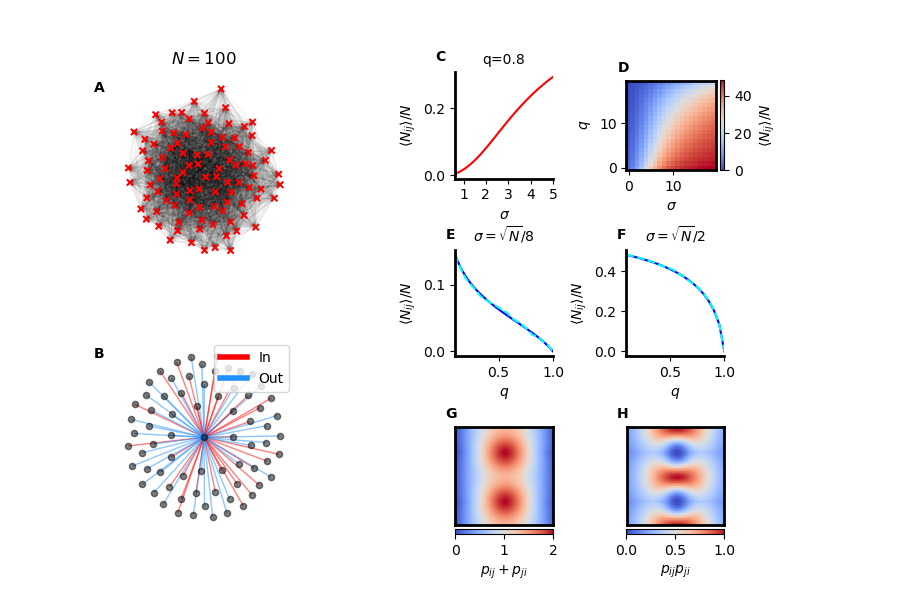
\includegraphics[width=175mm]{figure-8}
\caption{\textbf{The homogeneous Gaussian network}. (A) An example homogeneous network containing $N=100$ neurons. (B) An example neuron extracted from (A) with outgoing synapses labeled in blue and incoming synapses labeled in red. (C,D) The ratio $\langle N_{ij}\rangle/N$ as a function parameters ($\sigma, \Gamma_{0}$) for a sparse network (C) and a network with variable sparsity (D). (E,F) The ratio $\langle N_{ij}\rangle/N$ for fixed $\sigma$ and variable sparsity. (G,H) Binomial probability maps for two nearby neurons expressed as a sum $p_{ij}+p_{ji}$ and product $p_{ij}p_{ji}$}
\end{figure}

In other words, for the homogeneous case, the multiplication by $\gamma$ can be represented by a suitable selection of $\Gamma_{0}$ and can be set $\gamma=1$. Numerical evaluation of (3.7) shows that the ratio $\langle N_{ij}\rangle$ increases monotonically for increasing $\sigma$, as expected from (3.1b) and saturates at $\langle N_{ij}\rangle = 0.5$ at a rate proportional to $\sigma$. This can be understood from the fact that as $\Gamma_{0} \rightarrow 1$ we have $p_{0} \rightarrow 0$ and the multinomial distribution in (3.2) is reduced to a binomial distribution with $p_{ij} = p_{ji} = 1/2$. 

Furthermore, in addition to the average degree of a neuron, we are interested in the average number of shared inputs (outputs) between two neurons. We expect that this statistic makes at least a partial contribution to pairwise correlations in the voltage dynamics between two cells. To address this, we consider the average number of shared connections $\langle S_{ij} \rangle$ between a neuron $i$ and $j$ as a function of their distance $|\Delta \mathbf{r}_{ij}|$. In essence, this is the product $p_{ik}\cdot p_{jk}$ for a third neuron $k$ with $i,j\neq k$. The symmetry present in the homogeneous case allows us to perform this computation rather easily,

\begin{align}
\langle S_{ij} \rangle &= \frac{1}{N}\sum_{k} p_{ik}\cdot p_{jk} \\
&= \frac{\left(1-\Gamma_{0}\right)^{2}}{N}\sum_{k}\frac{\Gamma_{ik}(1-\Gamma_{ki})\Gamma_{jk}(1-\Gamma_{kj})}{Z_{ik}Z_{jk}}
\end{align}


which can be carried out numerically over the two-dimensions of space. Self-consistent with our definition of the connectivity kernel, the normalized number of shared connections decays with a gaussian profile for increasing $|\Delta \mathbf{r}_{ij}|$ as can be seen in Fig. (3.3).


 
\clearpage
\begin{figure}[t!]
\centering
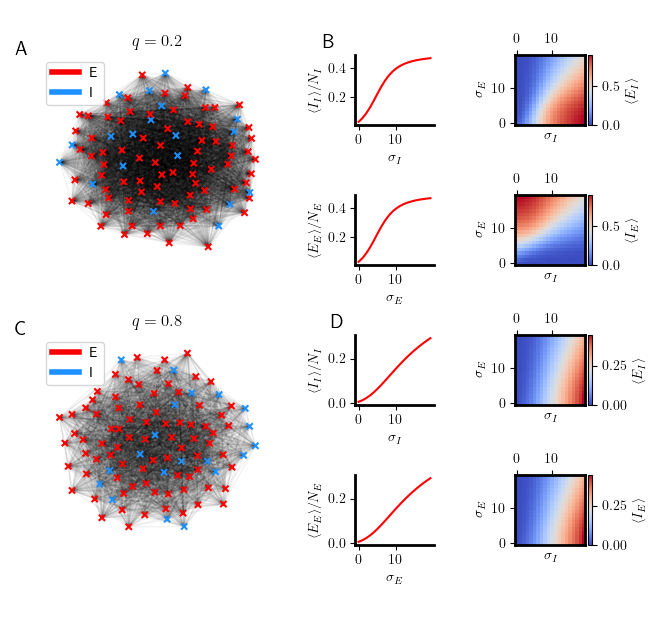
\includegraphics[width=165mm]{figure-9}
\caption{\textbf{Average degree in an excitatory-inhibitory network} (A) Schematic illustrating the notation used for excitatory-excitatory, excitatory-inhibitory, inhibitory-excitatory, and inhibitory-inhibitory synapses. (B) An example dense excitatory-inihbitory network ($\Gamma_{0}=0.2$) and $p_{E} = 0.8$. (C) Average number of synapses in the dense network normalized to the target population size as a function of parameters $\sigma_{E}$ and $\sigma_{I}$. (D) An example sparse excitatory-inihbitory network ($\Gamma_{0}=0.8$) and $p_{E} = 0.8$. (E) Average number of synapses in the sparse network normalized to the target population size as a function of parameters $\sigma_{E}$ and $\sigma_{I}$.}
\end{figure}


\section{Methods}


\subsection{Signal processing techniques}

The cross-correlation of discrete signals $x(t)$ and $y(t)$ is generally defined as the following convolution in the time-domain

\begin{align}
R_{xy}(\tau) = x(t) * y(t) = \sum_{k =-\infty}^{\infty}x(t)y(t+\tau)
\end{align}

where the $*$ symbol represents the convolution operation. Let $\psi_{x}(\omega)$ be the discrete-time Fourier transform (DTFT) of $x(t)$ i.e.,

\begin{align}
\psi_{x}(\omega) = \sum_{t =-\infty}^{\infty}x(t)\left(\exp{-i\omega t}\right)
\end{align}

where an identical expression exists for $\psi_{y}(\omega)$. According to the convolution theorem, convolution in the time-domain is equivalent to multiplication in the frequency domain with one of the signals time-reversed. Therefore, we can write

\begin{align}
\mathrm{DTFT}[x(t) * y(t)](\omega) = \underset{T\rightarrow\infty}{\mathrm{lim}}\frac{1}{2\pi T}\psi_{x}^{*}(\omega)\psi_{y}(\omega)
\end{align}


Let $S_{xy}(\omega) = \underset{T\rightarrow\infty}{\mathrm{lim}}\frac{1}{2\pi T}\psi_{x}^{*}(\omega)\psi_{y}(\omega)$, which is commonly called the \emph{cross spectral density} of signals $x(t)$ and $y(t)$. This is simply the DTFT of the cross-correlation function meaning that $R_{xx}(\tau)$ and $S_{xx}(\omega)$ form a Fourier pair. This result provides us an efficient means of computing cross-correlations and autocorrelations of synaptic currents by multiplication in the frequency domain and taking the inverse discrete transform.

\begin{align}
\mathbb{P} = \frac{p_{n}\prod_{m\neq n}(1-p_{m})}{\sum_{n}p_{n}\prod_{m\neq n}(1-p_{m})} = \frac{p_{n}\prod_{m\neq n}(1-p_{m})}{Z}
\end{align}

\subsection{Generating spatially extended networks}

where $Z$ is a normalization constant. For generating synapses, the probabilities of (3.1) are the probabilities over the possible synaptic states between $i$ and $j$

\begin{equation}
    \mathbb{P} = \left\{\begin{array}{lr}
        p_{ij} = \Gamma_{ij}(1-\Gamma_{ji})(1-\Gamma_{0})\cdot Z^{-1}\\
        p_{ji} = \Gamma_{ji}(1-\Gamma_{ij})(1-\Gamma_{0})\cdot Z^{-1}\\
        p_{0} = \Gamma_{0}(1-\Gamma_{ij})(1-\Gamma_{ji})\cdot Z^{-1}\\
        \end{array}\right\}
\end{equation}

\begin{align*}
Z = \Gamma_{ij}(1-\Gamma_{ji})(1-\Gamma_{0}) + \Gamma_{ji}(1-\Gamma_{ij})(1-\Gamma_{0}) + \Gamma_{0}(1-\Gamma_{ij})(1-\Gamma_{ji})
\end{align*}

Sampling from the distribution $\mathbb{P}$ for each of the $N^{2} - N$ possible synapses (excluding autapses), we can generate an asymmetric adjacency matrix $\mathcal{C} \in \mathbb{F}_{2}^{N\times N}$. An element $\mathcal{C}_{ij} = 1$ defines a synapse from $i\rightarrow j$ and $\mathcal{C}_{ji} = 1$ defines a synapse from $j\rightarrow i$.

Defining the generation of network connectivity in this way proves useful upon the realization that the network can be described by binomial statistics, similar to the well-known Erdos-Renyi (ER) random graph. Graph theory provides a rich set of metrics that can be used to discuss the statistical properties of the network defined by $\mathcal{C}$ and in turn the chosen kernel $\Gamma$. Assuming that we can compute the probabilities $p_{ij}, p_{ji}$ and $p_{0}$ for a particular $\Gamma$ and every synapse is generated independently, the mean of the out-degree distribution is

\begin{equation}
\langle N_{ij} \rangle = \sum_{j} \Gamma_{ij}(1-\Gamma_{ji})(1-\Gamma_{0})\cdot Z^{-1}
\end{equation}

where the spatial dependence of the individual kernels is implied. The in-degree distribution is found by simply swapping $i$ and $j$. The variance of the out-degree distribution is then

\begin{align}
\mathrm{Var}(N_{ij}) &= \sum_{j} \langle N_{ij}^{2} \rangle - \langle N_{ij} \rangle ^{2} \\
&= \sum_{j} \langle N_{ij}\rangle - \langle N_{ij} \rangle ^{2} 
\end{align}

from the linearity of variance property. We will analyze the in-degree and out-degree distributions of a graph generated when the connectivity kernel is a symmetric Gaussian extending over two-dimensions. We refer to this case as a \emph{two-dimensional gaussian network}.

The following model for generating the backbone for network of neurons rests on the assumption that we can create connectivity solely from pairwise connection probabilities. Let us define a spatial connectivity kernel $\Gamma_{i}(\mathbf{r}_{j})$ with $i,j\in \{n\}_{n=1}^{N}$ which defines the binomial probability that a neuron $i$ synapses onto a different cell $j\neq i$ at spatial coordinate $\mathbf{r}_{j}$. Here, the function $\Gamma_{i}(\mathbf{r})$ is not itself a probability distribution but rather represents one component of a distribution that is defined for each possible pairs $i,j$ for a given $i$. That distribution is completely represented for a pair $i,j$ with knowledge of the kernel $\Gamma_{j}(\mathbf{r}_{i})$ and an additional probability that no synapse occurs $\Gamma_{0}$. The parameter $\Gamma_{0}$ will be referred to as the $\emph{sparsity parameter}$ throughout the remainder of the text. Together, these three binomial probabilities can be renormalized to form a multinomial distribution $\mathbb{P}_{ij}$ at every possible synapse $ij$. A general definition of the multinomial distribution is

% Format a LaTeX bibliography
\makebibliography

[1] D.O. Hebb \textit{The organization of behavior: A neurophysiological theory}. John Wiley and Sons. 1949.

% Figures and tables, if you decide to leave them to the end
%\input{figure}
%\input{table}

\end{document}


